% UWaterloo ECE Work Term Report Template LaTeX source code
% Original Microsoft Word Document: <https://ece.uwaterloo.ca/~dwharder/Reports/Word/Report.Template.docx>
%
% Maintainer: Xin (Golson) Xie <golson.xie@uwaterloo.ca>
% Last Modified: 2014-06-28
% URL: <https://www.sharelatex.com/project/51b785e04c2bd70430657845>
% Documentation: <https://docs.google.com/document/d/1V9h24vhnaTfnRmiQWF3NaVye0RnbkpDhSldMcDREbNw>

% ******************************************************************************
% ********** Checklist: ********************************************************
% 
% Overall
% - 1.5" left margin and 1" top, right, and bottom margins
% - Full justification used for all paragraphs
% - 11-point default Roman font (by Knuth)
% - Section headings in 12- to 14-point default Roman font
% - 2 to 3 line spaces between sections
%
% Front Matter
% - No section or subsection numbering in front matter
% - 1.5 spacing except for the Letter of Submittal which is single spaced
% - Order: title page, letter of submittal, contributions, summary, table of
%   contents, list of figures, list of tables
% - Page numbers in lower case Roman numerals starting with iii for the
%   contributions
% - The table of contents, list of figures, and list of tables is appropriately
%   tab filled with ...... (dots)
% - The title page, letter of submittal, and table of contents does not appear
%   in the table of contents
% - List of figures appears on a separate page and contains all figures
%   appearing in the report body in the correct order
% - List of tables appears on a separate page and contains all tables appearing
%   in the report body in the correct order
% - The title page includes the university, faculty, and department names; the
%   title of the report, “Self Study” if it is a self-study report, the name and
%   location of the employer, the student’s full name, UW Student ID Number, and
%   UW User ID (engmail); the previously completed academic term, the completion
%   date of the report, and "Confidential-1" if the report is confidential
% 
% Body
% - 1.5 spacing
% - Restart page numbering at the start of the body
% - Sections, subsections, etc., are appropriately numbered in order
% - All figures have a number and a caption centred below the figure
% - All tables have a number and a caption centred above the table
% - The figure and table numbering are independent of each other and are
%   consistent in the report
% 
% Back Matter
% - Single spacing
% - No section numbers for the glossary or references (spelling error on
%   template)
% - Appendices are numbered using capital Latin letters
% ******************************************************************************

%%%%%%%%%%%%%%%%%%%%%%%%%%%%%%%%%%%%%%%%%%%%%%%%%%%%%%%%%%%%%%%%%%%%%%%%%%%%%%%%
%% ************************************************************************** %%
%% *                                Settings                                * %%
%% ************************************************************************** %%
%%%%%%%%%%%%%%%%%%%%%%%%%%%%%%%%%%%%%%%%%%%%%%%%%%%%%%%%%%%%%%%%%%%%%%%%%%%%%%%%

\documentclass{ece}
\loadglsentries{gls}
\glsaddall
\addbibresource{reference}

%%%%%%%%%%%%%%%%%%%%%%%%%%%%%%%%%%%%%%%%%%%%%%%%%%%%%%%%%%%%%%%%%%%%%%%%%%%%%%%%
% Make sure the following block contains the correct information               %
%%%%%%%%%%%%%%%%%%%%%%%%%%%%%%%%%%%%%%%%%%%%%%%%%%%%%%%%%%%%%%%%%%%%%%%%%%%%%%%%
\reporttitle{Title of Report}
\selfstudy % comment this line if this is not a self study report 
\employername{Employer Name}
\employerstreetaddress{Employer Address}
\employerlocation{City, Provice, Country}
\authorname{Givenname Middlename Surname}
\studentnumber{2NNNNNNN}
\userid{dwharder}
\term{NX}
\program{Electrical or Computer Engineering}
\confidential{1} % comment this line if this is not a confidential report
\authorstreetaddress{Your Address}
\authorlocation{City, Province, Country}
\authorpostalcode{Postal Code}
%%%%%%%%%%%%%%%%%%%%%%%%%%%%%%%%%%%%%%%%%%%%%%%%%%%%%%%%%%%%%%%%%%%%%%%%%%%%%%%%
% end of information block...                                                  %
%%%%%%%%%%%%%%%%%%%%%%%%%%%%%%%%%%%%%%%%%%%%%%%%%%%%%%%%%%%%%%%%%%%%%%%%%%%%%%%%

\begin{document}

%%%%%%%%%%%%%%%%%%%%%%%%%%%%%%%%%%%%%%%%%%%%%%%%%%%%%%%%%%%%%%%%%%%%%%%%%%%%%%%%
%% ************************************************************************** %%
%% *                               Title Page                               * %%
%% ************************************************************************** %%
%%%%%%%%%%%%%%%%%%%%%%%%%%%%%%%%%%%%%%%%%%%%%%%%%%%%%%%%%%%%%%%%%%%%%%%%%%%%%%%%

\maketitle

%%%%%%%%%%%%%%%%%%%%%%%%%%%%%%%%%%%%%%%%%%%%%%%%%%%%%%%%%%%%%%%%%%%%%%%%%%%%%%%%
%% ************************************************************************** %%
%% *                           Letter of Submittal                          * %%
%% ************************************************************************** %%
%%%%%%%%%%%%%%%%%%%%%%%%%%%%%%%%%%%%%%%%%%%%%%%%%%%%%%%%%%%%%%%%%%%%%%%%%%%%%%%%

\letterofsubmittal

\printauthorstreetaddress\\
\printauthorlocation\\
\printauthorpostalcode

\today

Manoj Sachdev, chair\\
Electrical and Computer Engineering\\
University of Waterloo\\
Waterloo, Ontario\\
N2L 3G1

Dear Sir:

This report, entitled ``Report Title'' was prepared as my \printterm Work Report for the University of Waterloo. This report is in fulfillment of the course \gls{wkrpt} N0N. The purpose of this report is... .  It is a self-study and confidential-1 report.

This is a one- or two-sentence paragraph describing the activities and objects of your employer.

This is a one- or two-sentence paragraph describing the group or department with whom you were employed, your manager, and the objects of that group.  This report was written for ... .

An acknowledgment of any assistance you received.  I hereby confirm that I have received no further help other than what is mentioned above in writing this report. I also confirm this report has not been previously submitted for academic credit at this or any other academic institution.

Sincerely,
\vspace*{6\baselineskip}

\printauthorname\\
\printstudentnumber

%%%%%%%%%%%%%%%%%%%%%%%%%%%%%%%%%%%%%%%%%%%%%%%%%%%%%%%%%%%%%%%%%%%%%%%%%%%%%%%%
%% ************************************************************************** %%
%% *                              Contributions                             * %%
%% ************************************************************************** %%
%%%%%%%%%%%%%%%%%%%%%%%%%%%%%%%%%%%%%%%%%%%%%%%%%%%%%%%%%%%%%%%%%%%%%%%%%%%%%%%%

\contributions

This is a self-study work-term report not based on the experienced gained at my previous co-op job.  The team I worked with was relatively small or large... .  It falls within the X group.  It consisted of N people.

The team's main goal or goals were... .

My task or tasks were... .  \emph{or}  My task or tasks consisted of... .

The relationship between this report and my job... .

In the broader scheme of things, ... .

%%%%%%%%%%%%%%%%%%%%%%%%%%%%%%%%%%%%%%%%%%%%%%%%%%%%%%%%%%%%%%%%%%%%%%%%%%%%%%%%
%% ************************************************************************** %%
%% *                                Summary                                 * %%
%% ************************************************************************** %%
%%%%%%%%%%%%%%%%%%%%%%%%%%%%%%%%%%%%%%%%%%%%%%%%%%%%%%%%%%%%%%%%%%%%%%%%%%%%%%%%

\summary

The main purpose of the report is... .  \emph{or}  The scope of the report is... .

The major points documented/covered in this report are... .

The major conclusions in this report are... .

The major recommendations in this report are... .

%%%%%%%%%%%%%%%%%%%%%%%%%%%%%%%%%%%%%%%%%%%%%%%%%%%%%%%%%%%%%%%%%%%%%%%%%%%%%%%%
%% ************************************************************************** %%
%% *                           Table of Contents                            * %%
%% ************************************************************************** %%
%%%%%%%%%%%%%%%%%%%%%%%%%%%%%%%%%%%%%%%%%%%%%%%%%%%%%%%%%%%%%%%%%%%%%%%%%%%%%%%%

\tableofcontents

%%%%%%%%%%%%%%%%%%%%%%%%%%%%%%%%%%%%%%%%%%%%%%%%%%%%%%%%%%%%%%%%%%%%%%%%%%%%%%%%
%% ************************************************************************** %%
%% *                            List of Figures                             * %%
%% ************************************************************************** %%
%%%%%%%%%%%%%%%%%%%%%%%%%%%%%%%%%%%%%%%%%%%%%%%%%%%%%%%%%%%%%%%%%%%%%%%%%%%%%%%%

\listoffigures

%%%%%%%%%%%%%%%%%%%%%%%%%%%%%%%%%%%%%%%%%%%%%%%%%%%%%%%%%%%%%%%%%%%%%%%%%%%%%%%%
%% ************************************************************************** %%
%% *                             List of Tables                             * %%
%% ************************************************************************** %%
%%%%%%%%%%%%%%%%%%%%%%%%%%%%%%%%%%%%%%%%%%%%%%%%%%%%%%%%%%%%%%%%%%%%%%%%%%%%%%%%

\listoftables

%%%%%%%%%%%%%%%%%%%%%%%%%%%%%%%%%%%%%%%%%%%%%%%%%%%%%%%%%%%%%%%%%%%%%%%%%%%%%%%%
%% ************************************************************************** %%
%% *                                  Body                                  * %%
%% ************************************************************************** %%
%%%%%%%%%%%%%%%%%%%%%%%%%%%%%%%%%%%%%%%%%%%%%%%%%%%%%%%%%%%%%%%%%%%%%%%%%%%%%%%%

\body

\section{Introduction}

This is the introduction.

\subsection{Subsection}

Some more text and a cross reference to \Cref{app:firstappx} and remember that one can lie about statistics \cite{liewithstat}.

\subsubsection{Sub-subsection}

% consistent figure numbering in the report body
This section will demonstrate figures.  \Cref{fig:wine} shows the result of storing a bottle of white wine for sixteen years.

% all figures have a number and title/caption below the figure
\begin{figure}[ht!] % h! means "here!" (instead of on top of the page)
    \centering 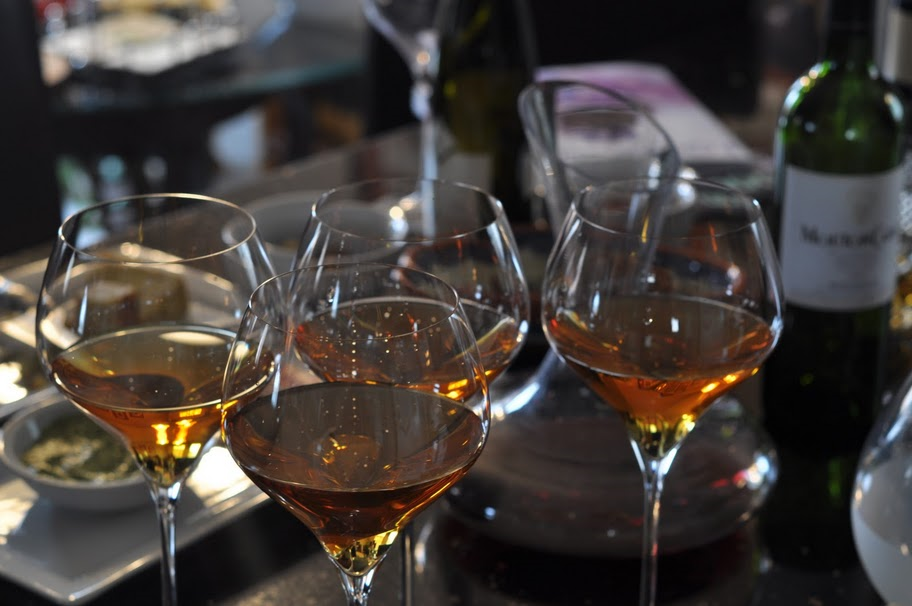
\includegraphics[width=0.5\textwidth]{wine}
    \caption{16-year old white wine.}
    \label{fig:wine}
\end{figure}

The wine becomes deeper in colour going from a light yellow to golden.
\subsubsection{Another Sub-subsection}

% consistent table numbering in the report body
Some more text.  As a demonstration of tables, \Cref{tab:numbertable} demonstrates how certain types of entries should appear in a table.  Note that, in order to centre the numbers in the last column, three columns are given.

% tables have a number and title/caption above the table
\begin{table}[ht!] % h! means "here!" (instead of on top of the page)
    \caption{A table of numbers}
    \label{tab:numbertable}
    \centering
    \begin{tabular}{l r c r l S[table-format=5.4]}
        % 4.4 means 4 digits before and after the decimal point
        
        \hline
              & \multicolumn{1}{c}{\textbf{Integers}} & \multicolumn{1}{c}{\textbf{Boolean}} & \multicolumn{1}{c}{\textbf{Monetary}} & \multicolumn{1}{c}{\textbf{Text}} & \multicolumn{1}{c}{\textbf{Units (g/mL)}} \\
        \hline
        % ~ gives space
        Row 1   & 3~~~      & T & 12.34     & First class       & 0.1234 \\
        Row 2   & 9~~~      & F & 5.67      & Some more text    & 5.67 \\
        Row 3   & 23~~~     & F & 890.12    & Other text        & 89.01 \\
        Row 4   & 157~~~    & T & 34.56     & Even more text    & 23456.7 \\
        \hline
    \end{tabular}
\end{table}

\subsection{Another Subsection}

Some more text.

\subsection{A Third Subsection}

Some text and a reference to \Cref{app:anotherappx} which contains additional information related to this report.

\section{Background}

% consistent table numbering in the report body
The background of the report.  As another example, \Cref{tab:anothernumbertable} displays another set of numbers, but are actually the same as \Cref{tab:numbertable}.

% tables have a number and title/caption above the table
\begin{table}[ht!]
    \caption{Another table of numbers}
    \label{tab:anothernumbertable}
    \centering
    \begin{tabular}{l r c r l S[table-format=5.4]}
        % 4.4 means 4 digits before and after the decimal point
        
        \hline
              & \multicolumn{1}{c}{\textbf{Integers}} & \multicolumn{1}{c}{\textbf{Boolean}} & \multicolumn{1}{c}{\textbf{Monetary}} & \multicolumn{1}{c}{\textbf{Text}} & \multicolumn{1}{c}{\textbf{Units (g/mL)}} \\
        \hline
        Row 1 & 3~~~                                  & T                                    & 12.34                                 & First class                       & 0.1234                                    \\
        Row 2 & 9~~~                                  & F                                    & 5.67                                  & Some more text                    & 5.67                                      \\
        Row 3 & 23~~~                                 & F                                    & 890.12                                & Other text                        & 89.01                                     \\
        Row 4 & 157~~~                                & T                                    & 34.56                                 & Even more text                    & 23456.7                                   \\
        \hline
    \end{tabular}
\end{table}

\section{The Engineering Problem}

Some more text.

\section{Requirements, Criteria, and Metrics}

% add when necessary
\label{sec:rcm} % a label for "requirement, criteria, and metrics"

A list of the requirements, criteria and metrics that will be used in this report together with a discussion on any issues surrounding the selection of these.

This is an example of an inline equation: the formula $\sum_{n=1}^{\infty}\frac{1}{n^2}=\frac{\pi^{2}}{6}$ is often taught in first year.  The integral, however, is slightly less, as is shown by the display equation

\begin{center}
    $\int\limits_{1}^{\infty}\frac{1}{x^{2}}\, \mathrm{d}x=1$.
\end{center}

This is of course centred.

\section{Possible Solutions}

Equations can be numbered, for example, it may be necessary to refer to

\begin{equation}
    \label{eq:newtonssecondlaw}
    F=\frac{\mathrm{d}}{\mathrm{d}t}(m\mathbf{v}),
\end{equation}

that is, Newton\textquoteright s second law, elsewhere in the document.  Cut-and-paste this table if you require an equation elsewhere.

\subsection{Solution 1}

A description and discussion of solution 1 and a reference to \cref{eq:newtonssecondlaw}.

\subsection{Solution 2}

A description and discussion of solution 2.

\subsection{Solution 3}

A description and discussion of solution 3 and so on.

\section{Engineering Analysis}

The analysis of the solutions based on the requirements and criteria listed above based on the metrics listed in \Cref{sec:rcm} on \cpageref{sec:rcm}

\section*{Conclusions}

From the analysis in the report body, it was concluded that...

\section*{Recommendations}

Based on the analysis and conclusions in this report, it is recommended that...

%%%%%%%%%%%%%%%%%%%%%%%%%%%%%%%%%%%%%%%%%%%%%%%%%%%%%%%%%%%%%%%%%%%%%%%%%%%%%%%%
%% ************************************************************************** %%
%% *                                Glossary                                * %%
%% ************************************************************************** %%
%%%%%%%%%%%%%%%%%%%%%%%%%%%%%%%%%%%%%%%%%%%%%%%%%%%%%%%%%%%%%%%%%%%%%%%%%%%%%%%%

\printglossaries

%%%%%%%%%%%%%%%%%%%%%%%%%%%%%%%%%%%%%%%%%%%%%%%%%%%%%%%%%%%%%%%%%%%%%%%%%%%%%%%%
%% ************************************************************************** %%
%% *                               References                               * %%
%% ************************************************************************** %%
%%%%%%%%%%%%%%%%%%%%%%%%%%%%%%%%%%%%%%%%%%%%%%%%%%%%%%%%%%%%%%%%%%%%%%%%%%%%%%%%

\printbibliography[heading=none]

%%%%%%%%%%%%%%%%%%%%%%%%%%%%%%%%%%%%%%%%%%%%%%%%%%%%%%%%%%%%%%%%%%%%%%%%%%%%%%%%
%% ************************************************************************** %%
%% *                               Appendices                               * %%
%% ************************************************************************** %%
%%%%%%%%%%%%%%%%%%%%%%%%%%%%%%%%%%%%%%%%%%%%%%%%%%%%%%%%%%%%%%%%%%%%%%%%%%%%%%%%

% appendices use section and subsection numbering
\appendix

\section{Title of First Appendix}
\label{app:firstappx}
Use the No Spacing style.

\section{Another Appendix}
\label{app:anotherappx}
Again, use the no spacing style for appendices.

\end{document}
